\documentclass[12pt]{scrartcl}

\usepackage[utf8]{inputenc}
\usepackage[IL2]{fontenc}
\usepackage[czech]{babel}
\usepackage{graphicx}
\usepackage{hyperref}
\usepackage{amsmath}
\usepackage[]{algorithm2e}
\usepackage{enumitem}
\usepackage{gensymb}

\subject{Západočeská univerzita v\nobreakspace Plzni\\Fakulta aplikovaných věd\\KIV/KPG}
\author{Pavel Zelenka\\A16B0176P\\zelenkap@students.zcu.cz}
\date{\today}
\title{Spline křivka}

\begin{document}
\maketitle
\pagenumbering{gobble}
\newpage
\pagenumbering{arabic}
\newpage
\section{Zadání}
	
\paragraph{}
Zadáním úkolu je vytvoření nového programu nebo rozšíření programu ze cvičení, aby umožňoval vykreslení libovolné námi zvolené spline křivky - kromě Beziérovy křivky.

\section{Analýza problému}

\paragraph{}
\textbf{Spline} je\nobreakspace aproximační křivka, která je\nobreakspace obvykle dána množinou \textbf{řídících bodů}. Křivka je\nobreakspace popsána pomocí polynomů, její vlastností je tedy diferencovatelnost, křivka je\nobreakspace \textbf{hladká}. Křivka může být interpolací, kdy prochází všemi řídícími body nebo jen\nobreakspace aproximací, kdy řídící body určují tvar, ale\nobreakspace křivka jimi nemusí procházet.

\paragraph{}
V této práci se nudu zabývat \textbf{B-spline křivkou} a \textbf{kubickou spline křivkou}, které budou implementovány v odevzdávané aplikaci. Obě křivky budou využívat kubický polynom (tj. polynom třetího stupně $y = a + bx + cx^2 + dx^3$ ).


\section{Popis řešení}

\paragraph{}
Vykreslování probíhá ve\nobreakspace třídě \emph{Drawing}. Křivky\nobreakspace  se nacházejí v balíčku \emph{splines}. Aplikace nabízí pouze křivky z výčtového typu \emph{SplineType}, kde musí být uvedeny všechny dostupné křivky z aplikace.\\

\subsection{B-spline křivka}
\paragraph{}
\begin{algorithm}[H]
\KwIn{řídící body, počet kroků}
	křivka = prázdný seznam bodů\;
	nový bod = null\;
	předchozí bod = null\;
	první = true\;
	n = počet řídících bodů\;
	\For{i = 1; i $<$ n-2; n+1} {
		a = řídící bod na pozici i-1\;
		b = řídící bod na pozici i\;
		c = řídící bod na pozici i+1\;
		d = řídící bod na pozici i+2\;
		s3 = nový bod $\left[ \frac{-a_x + 3 \cdot (b_x - c_x + d_x)}{6}, \frac{-a_y + 3 \cdot (b_y - c_y + d_y)}{6} \right] $\;
		s2 = nový bod $\left[ \frac{a_x - 2 \cdot b_x + c_x}{2}, \frac{a_y - 2 \cdot b_y + c_y}{2} \right] $\;		
		s1 = nový bod $\left[ \frac{c_x - a_x}{2}, \frac{c_y - a_y}{2} \right] $\;				
		s0 = nový bod $\left[ \frac{a_x + 4 \cdot b_x + c_x}{6}, \frac{a_y + 4 \cdot b_y + c_y}{6} \right] $\;			
		\For{krok = 0; krok $<=$ počet kroků; krok+1} {
			předchozí bod = nový bod\;
			t = krok / počet kroků\;
			nový bod = $\left[ a_x + t \cdot \left( b_x + t \cdot \left( c_x + t \cdot d_x \right) \right), a_y + t \cdot \left( b_y + t \cdot \left( c_y + t \cdot d_y \right) \right) \right] $\;
		\eIf{první}
			{
			první = false\;
			}
			{
				přidat nový bod do křivky\;
				přidat předchozí bod do křivky\;
			}
		}
	}
 \Return{křivka}
 \caption{Výpočet B-spline křivky}
\end{algorithm}

\subsection{Kubická spline křivka}
\paragraph{}
\begin{algorithm}[H]
\KwIn{řídící body, počet kroků}
 bod$[\nobreakspace ]$ = kopie seznamu řídících bodů\;
 n$[\nobreakspace ]$ = počet řídících bodů-1\;
 gamma$[\nobreakspace ]$ = pole čísel velikosti n+1\;
 delta$[\nobreakspace ]$ = pole bodů velikosti n+1\;
 D$[\nobreakspace ]$ = pole bodů velikosti n+1\;
 gamma$[0]$ = 0.5\;
 \For{i = 1; i $<$ n; i+1} {
   gamma$[i]$ = $\frac{1}{4 - gamma[i-1]}$ \;
 }
 gamma$[n]$ = $\frac{1}{2 - gamma[n-1]}$\;
 delta$[0]$ = nový bod $[ 3 \cdot (bod[1]_x - bod[0]_x) \cdot gamma[0], $ \\ \nobreakspace \nobreakspace \nobreakspace \nobreakspace \nobreakspace $  3 \cdot (bod[1]_y - bod[0]_y) \cdot gamma[0] ] $\; 
 \For{i = 1; i $<$ n; i+1} {
    delta$[i]$ = nový bod $[ 3 \cdot (bod[i+1]_x - bod[i-1]_x) - delta[i-1]_x \cdot gamma[i],$ \\ \nobreakspace \nobreakspace \nobreakspace \nobreakspace \nobreakspace $ 3 \cdot (bod[i+1]_y - bod[i-1]_y) - delta[i-1]_y \cdot gamma[i] ] $\;
 }
 delta$[n]$ = nový bod $[ 3 \cdot (bod[n]_x - bod[n-1]_x - delta[n-1]_x) \cdot gamma[n],$ \\ \nobreakspace \nobreakspace \nobreakspace \nobreakspace \nobreakspace $ 3 \cdot (bod[n]_y - bod[n-1]_y - delta[n-1]_y) \cdot gamma[n]] $\;
 \For{i = n; i $>=$ 0; i-1} {
 	D$[i]$ = nový bod $[delta[i]_x - gamma[i] \cdot D[i + 1]_x, delta[i]_y - gamma[i] \cdot D[i + 1]_y] $
 }
 \For{i = 1; i $<$ n; i+1} {
   a = nový bod $[bod[i]_x, bod[i]_y]$ \;
   b = nový bod $[D[i]_x, D[i]_y]$ \;
   c = nový bod $[ 3 \cdot (bod[i+1]_x - bod[i]_x) - 2 \cdot D[i]_x - D[i+1]_x,$ \\ \nobreakspace \nobreakspace \nobreakspace \nobreakspace \nobreakspace $ 3 \cdot (bod[i+1]_y - bod[i]_y) - 2 \cdot D[i]_y - D[i+1]_y ]$\;
   d = nový bod $[ 2 \cdot (bod[i]_x - bod[i+1]_x) + D[i]_x + D[i+1]_x,$ \\ \nobreakspace \nobreakspace \nobreakspace \nobreakspace \nobreakspace $ 2 \cdot (bod[i]_y - bod[i+1]_y) + D[i]_y + D[i+1]_y ]$\;
 \For{krok = 0; krok $<=$ počet kroků; krok+1} {
   t = krok / počet kroků\;
   nový bod = $\left[ a_x + t \cdot \left( b_x + t \cdot \left( c_x + t \cdot d_x \right) \right), a_y + t \cdot \left( b_y + t \cdot \left( c_y + t \cdot d_y \right) \right) \right] $\;
   přidat nový bod do křivky\;
  }
 }
 \Return{křivka}
 \caption{Výpočet kubické spline křivky}
\end{algorithm}

\newpage
\section{Uživatelská dokumentace}

\paragraph{}
Spuštění aplikace se\nobreakspace provede souborem \texttt{Spline.jar}, který se nachází ve složce \emph{App}.

\paragraph{}
Po\nobreakspace spuštění aplikace se\nobreakspace zobrazí okno s plátném. Skrze pravé tlačítko myší lze na plátno přidávat nové řídící body křivky. Kliknutím levým tlačítkem na řídící bod se provede vybrání bodu, tažením myší pak lze bod přemístit. Plátno se automaticky uzpůsobí rozměrům okna a rozměrům křivky. Typ křivky, barvu a tloušťku lze měnit v\nobreakspace panelu v\nobreakspace dolní části okna. Křivku lze uložit jako rastrový obrázek formátu \texttt{PNG} kliknutím na tlačítko \texttt{Save As...} v nabídce \texttt{File}. Rozměry ukládaného obrázku se nastaví dle rozměrů křivky, pozadí obrázku bude průhledné. Plátno se vyčistí kliknutím na tlačítko \texttt{Clear}.

\begin{figure}[!ht]
	\centering
	\label{obr:polekolizi}
	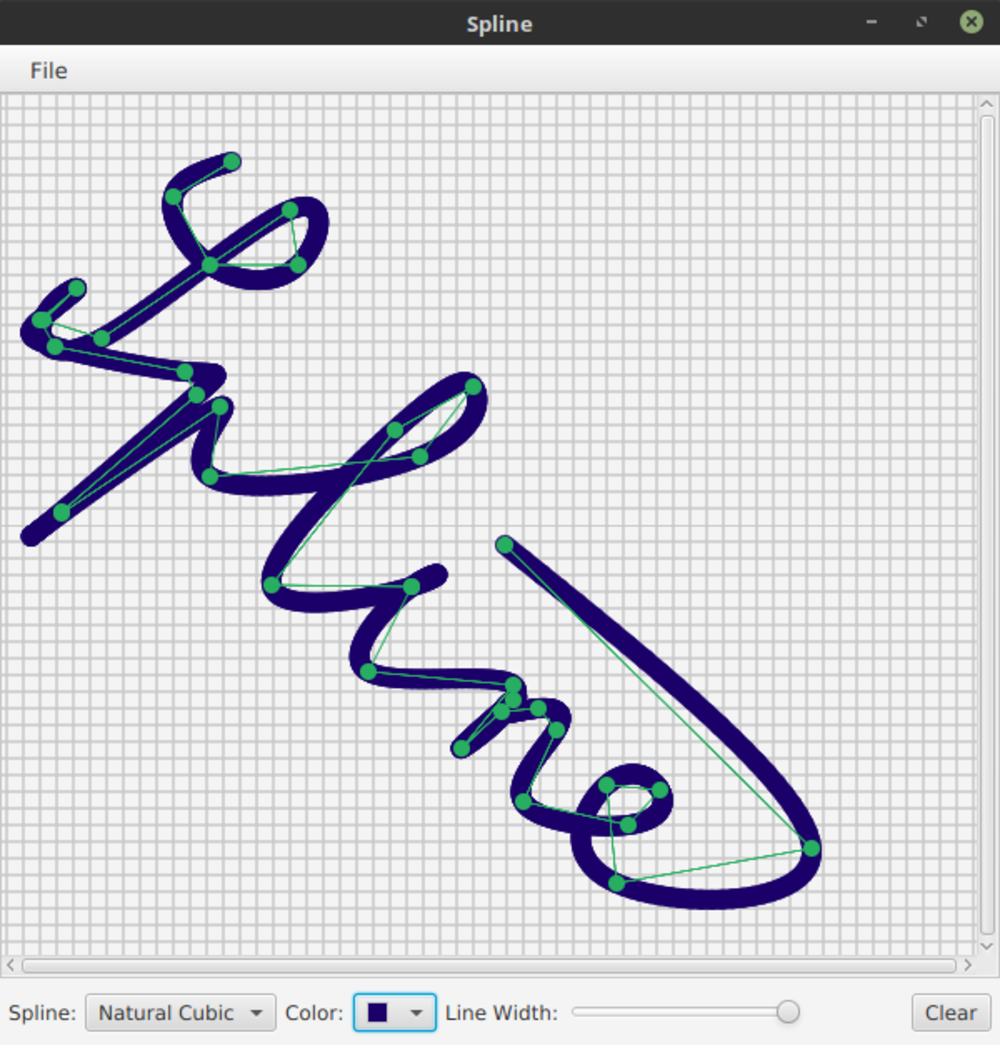
\includegraphics[width=0.85\textwidth,natwidth=1,natheight=1]{app_gui.pdf}
	\caption{Okno aplikace}
\end{figure}

\newpage
\section{Závěr}
\paragraph{}
Úkol jsem řešil v\nobreakspace jazyce \texttt{Java} s použitím grafických knihoven \texttt{JavaFX}. V knihovně JavaFX mi nevyhovovala implementace \texttt{Point2D}, kde není možná změna pozice existujícího bodu, proto je v odevdávané aplikaci vlastní implementace bodu. Nepodařilo\nobreakspace se\nobreakspace mi zjistit, zdali existuje řešení bez nutnosti vlastní implementace.
\paragraph{}
Aplikace v odevzdávané verzi obsahuje pouze b-spline a kubickou křivku, ovšem aplikace byla psána s ohledem pro snadné rozšíření o další typy spline křivek. 

\section{Reference}

Cubic Spline – Wolfram MathWorld. [online].\\ Dostupné z: \href{http://mathworld.wolfram.com/CubicSpline.html}{mathworld.wolfram.com/CubicSpline.html}

\end{document}
